% Source: Code/ML_overlay/ir_rgb_registration/paper/ml_overlay_report_materials/ir_rgb_registration_report/figures/fig_voxelmorph_architecture.tex
\documentclass[tikz,border=10pt]{standalone}
\usepackage{tikz}
\usetikzlibrary{positioning,shapes.geometric,arrows.meta,calc}

\definecolor{Garnet}{RGB}{115,0,10}
\definecolor{Rose}{RGB}{204,46,64}
\definecolor{Atlantic}{RGB}{70,106,159}
\definecolor{Congaree}{RGB}{31,65,77}
\definecolor{Horseshoe}{RGB}{101,120,11}
\definecolor{Black90}{RGB}{54,54,54}
\definecolor{Black70}{RGB}{92,92,92}

\begin{document}
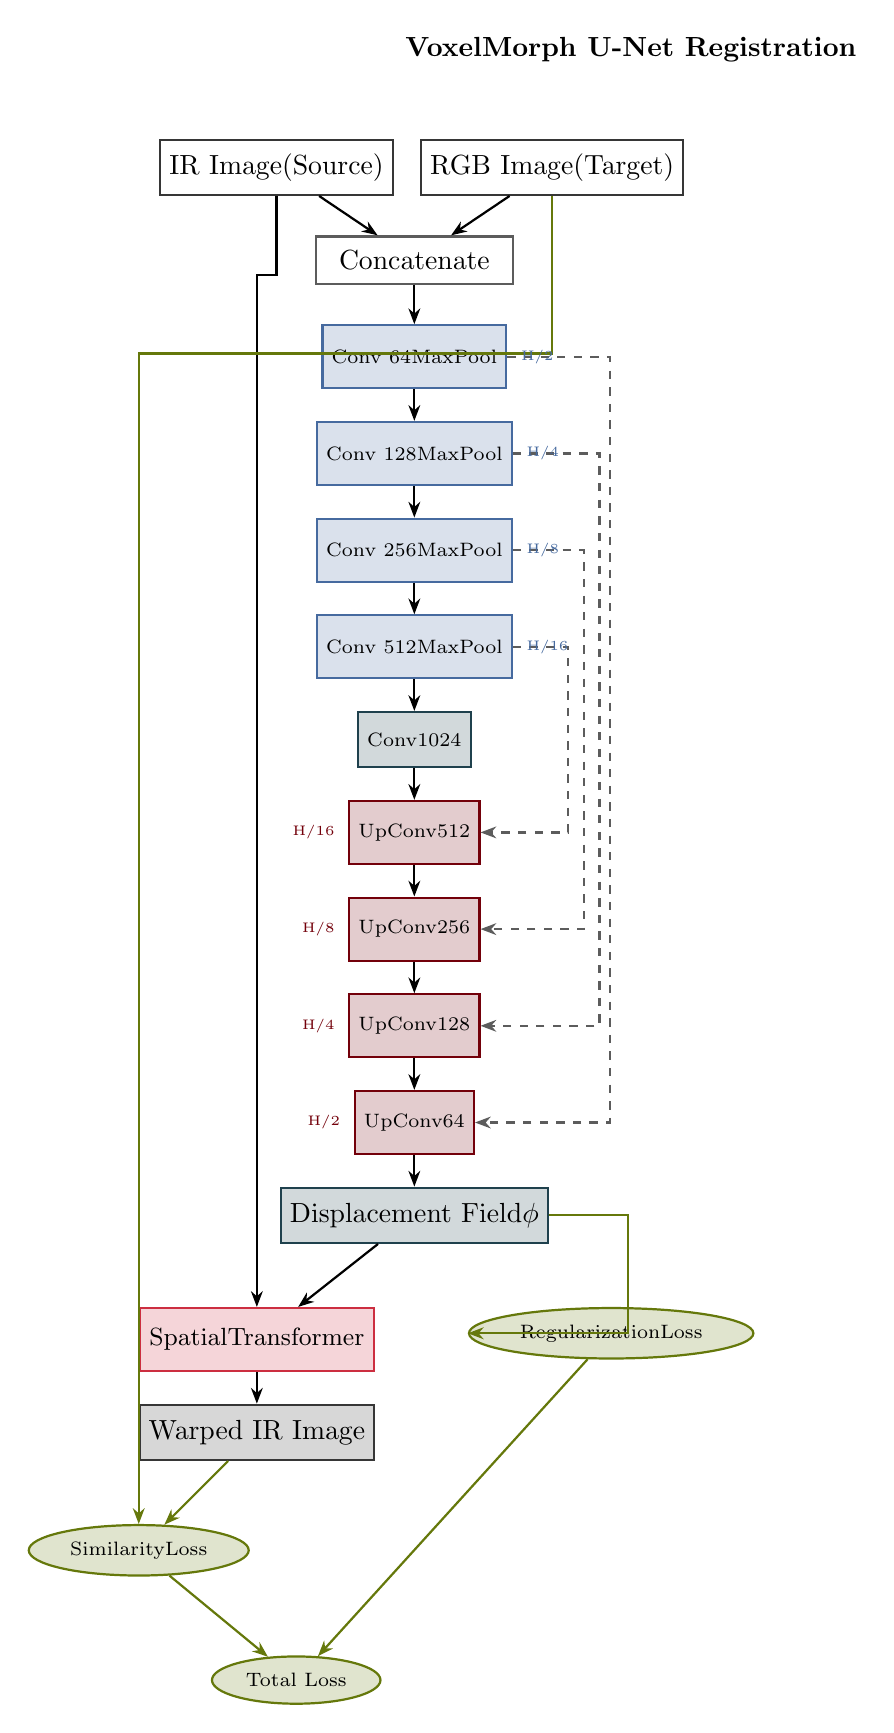
\begin{tikzpicture}[
    encoder/.style={rectangle,draw=Atlantic,fill=Atlantic!20,thick,minimum width=1.5cm,minimum height=0.8cm,font=\scriptsize},
    decoder/.style={rectangle,draw=Garnet,fill=Garnet!20,thick,minimum width=1.5cm,minimum height=0.8cm,font=\scriptsize},
    warp/.style={rectangle,draw=Rose,fill=Rose!20,thick,minimum width=1.8cm,minimum height=0.8cm,font=\small},
    loss/.style={ellipse,draw=Horseshoe,fill=Horseshoe!20,thick,minimum width=1.5cm,minimum height=0.6cm,font=\scriptsize},
    arrow/.style={-{Stealth[length=2mm]},thick}
]

\node[font=\bfseries] at (6,10) {VoxelMorph U-Net Registration};

% Input images
\node[rectangle,draw=Black90,thick,minimum width=1.8cm,minimum height=0.7cm] (ir-input) at (1.5,8.5) {IR Image\\(Source)};
\node[rectangle,draw=Black90,thick,minimum width=1.8cm,minimum height=0.7cm] (rgb-input) at (5,8.5) {RGB Image\\(Target)};

% Concatenate
\node[rectangle,draw=Black70,thick,minimum width=2.5cm,minimum height=0.6cm,below=0.5cm of rgb-input,xshift=-1.75cm] (concat) {Concatenate};
\draw[arrow] (ir-input) -- (concat);
\draw[arrow] (rgb-input) -- (concat);

% Encoder path (contracting)
\node[encoder,below=0.5cm of concat] (enc1) {Conv 64\\MaxPool};
\node[encoder,below=0.4cm of enc1,minimum width=1.3cm] (enc2) {Conv 128\\MaxPool};
\node[encoder,below=0.4cm of enc2,minimum width=1.1cm] (enc3) {Conv 256\\MaxPool};
\node[encoder,below=0.4cm of enc3,minimum width=0.9cm] (enc4) {Conv 512\\MaxPool};

\draw[arrow] (concat) -- (enc1);
\draw[arrow] (enc1) -- (enc2);
\draw[arrow] (enc2) -- (enc3);
\draw[arrow] (enc3) -- (enc4);

% Bottleneck
\node[rectangle,draw=Congaree,fill=Congaree!20,thick,minimum width=0.8cm,minimum height=0.7cm,font=\scriptsize,below=0.4cm of enc4] (bottleneck) {Conv\\1024};
\draw[arrow] (enc4) -- (bottleneck);

% Decoder path (expanding)
\node[decoder,below=0.4cm of bottleneck,minimum width=0.9cm] (dec4) {UpConv\\512};
\node[decoder,below=0.4cm of dec4,minimum width=1.1cm] (dec3) {UpConv\\256};
\node[decoder,below=0.4cm of dec3,minimum width=1.3cm] (dec2) {UpConv\\128};
\node[decoder,below=0.4cm of dec2,minimum width=1.5cm] (dec1) {UpConv\\64};

\draw[arrow] (bottleneck) -- (dec4);
\draw[arrow] (dec4) -- (dec3);
\draw[arrow] (dec3) -- (dec2);
\draw[arrow] (dec2) -- (dec1);

% Skip connections
\draw[arrow,dashed,Black70] (enc4.east) -- ++(0.7,0) |- (dec4.east);
\draw[arrow,dashed,Black70] (enc3.east) -- ++(0.9,0) |- (dec3.east);
\draw[arrow,dashed,Black70] (enc2.east) -- ++(1.1,0) |- (dec2.east);
\draw[arrow,dashed,Black70] (enc1.east) -- ++(1.3,0) |- (dec1.east);

% Output displacement field
\node[rectangle,draw=Congaree,fill=Congaree!20,thick,minimum width=2cm,minimum height=0.7cm,below=0.4cm of dec1] (disp-field) {Displacement Field\\$\phi$};
\draw[arrow] (dec1) -- (disp-field);

% Spatial transformer
\node[warp,below=0.8cm of disp-field,xshift=-2cm] (transformer) {Spatial\\Transformer};
\draw[arrow] (disp-field) -- (transformer);
\draw[arrow] (ir-input.south) -- ++(0,-1) -| (transformer.north);

% Warped output
\node[rectangle,draw=Black90,fill=Black90!20,thick,minimum width=2cm,minimum height=0.7cm,below=0.4cm of transformer] (warped) {Warped IR Image};
\draw[arrow] (transformer) -- (warped);

% Loss functions
\node[loss,below=0.8cm of warped,xshift=-1.5cm] (sim-loss) {Similarity\\Loss};
\node[loss,below=0.8cm of disp-field,xshift=2.5cm] (reg-loss) {Regularization\\Loss};

\draw[arrow,Horseshoe] (warped) -- (sim-loss);
\draw[arrow,Horseshoe] (rgb-input.south) -- ++(0,-2) -| (sim-loss.north);
\draw[arrow,Horseshoe] (disp-field.east) -- ++(1,0) |- (reg-loss.west);

% Total loss
\node[loss,below=1cm of sim-loss,xshift=2cm,minimum width=1.8cm] (total-loss) {Total Loss};
\draw[arrow,Horseshoe] (sim-loss) -- (total-loss);
\draw[arrow,Horseshoe] (reg-loss) -- (total-loss);

% Annotations
\node[font=\tiny,text=Atlantic,right=0.05cm of enc1] {H/2};
\node[font=\tiny,text=Atlantic,right=0.05cm of enc2] {H/4};
\node[font=\tiny,text=Atlantic,right=0.05cm of enc3] {H/8};
\node[font=\tiny,text=Atlantic,right=0.05cm of enc4] {H/16};
\node[font=\tiny,text=Garnet,left=0.05cm of dec4] {H/16};
\node[font=\tiny,text=Garnet,left=0.05cm of dec3] {H/8};
\node[font=\tiny,text=Garnet,left=0.05cm of dec2] {H/4};
\node[font=\tiny,text=Garnet,left=0.05cm of dec1] {H/2};

\end{tikzpicture}
\end{document}
